\label{result_har}

\subsubsection{Kết quả trên các bộ dữ liệu thử nghiệm}

\paragraph{Đánh giá trên tập dữ liệu riêng tư}

\begin{figure}[b!]
    \centering
    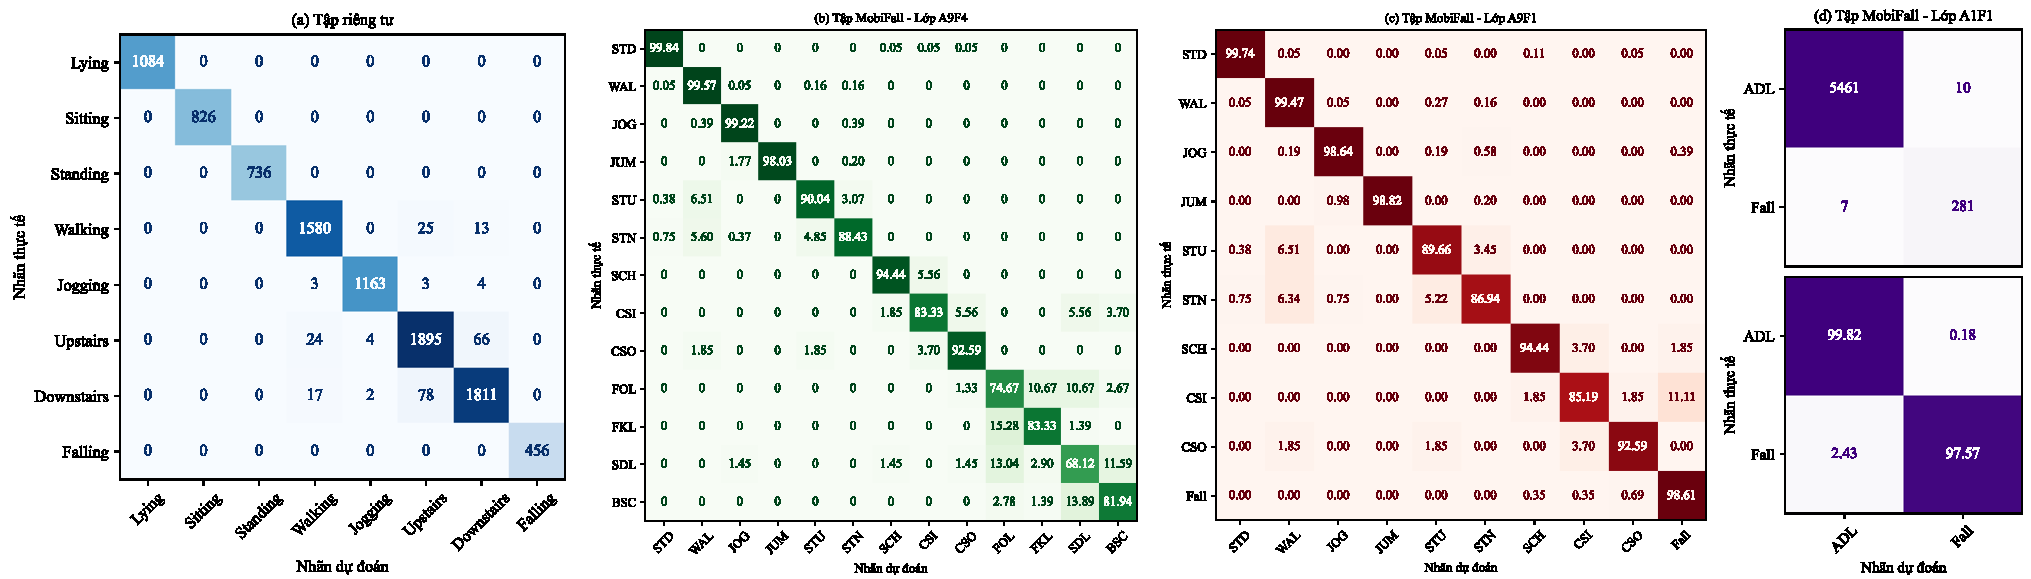
\includegraphics[width=1\linewidth]{Figure/confusion_matrices.pdf}
    \caption{Ma trận nhầm lẫn trên toàn bộ cơ sở dữ liệu: (a) Tập riêng tư; Tập MobiFall với (b) Tổ hợp A9F4, (c) Tổ hợp A9F1 và (d) Tổ hợp A1F1}
    \label{confusion_matrices}
\end{figure}

\begin{table}[t]
    \centering
    \caption{Báo cáo kết quả phân loại trên tập riêng tư và các tổ hợp A9F4, A9F1 trên tập MobiFall}
    \label{classification_report}
    \begin{tabular}{lccc||cccc||cccc}\hline\hline
        \multicolumn{4}{c||}{\textbf{Tập riêng tư}} & \multicolumn{4}{c||}{\textbf{Tập MobiFall - Tổ hợp A9F4}} & \multicolumn{4}{c}{\textbf{Tập MobiFall - Tổ hợp A9F1}}\\
        \textbf{Activity} & \textbf{PRE} & \textbf{SEN} & \textbf{F1} & \textbf{Activity} & \textbf{PRE} & \textbf{SEN} & \textbf{F1} & \textbf{Activity} & \textbf{PRE} & \textbf{SEN} & \textbf{F1}\\\hline
        Lying & 100 & 100 & 100 & STD & 99,79 & 99,84 & 99,81 & STD & 99,79 & 99,74 & 99,76\\
        
        Sitting & 100 & 100 & 100 & WAL & 98,16 & 99,57 & 98,86 & WAL & 98,05 & 99,47 & 98,75\\
        
        Standing & 100 & 100 & 100 & JOG & 97,70 & 99,22 & 98,46 & JOG & 98,45 & 98,64 & 98,54\\
        
        Walking & 97,29 & 97,65 & 97,47 & JUM & 100 & 98,03 & 99,01 & JUM & 100 & 98,82 & 99,41\\
        
        Jogging & 99,49 & 99,15 & 99,32 & STU & 93,25 & 90,04 & 91,62 & STU & 91,41 & 89,66 & 90,52\\
        
        Upstairs & 94,70 & 95,27 & 94,99 & STN & 94,42 & 88,43 & 91,33 & STN & 93,57 & 86,94 & 90,14\\
        
        Downstairs & 95,62 & 94,92 & 95,27 & SCH & 94,44 & 94,44 & 94,44 & SCH & 92,73 & 94,44 & 93,58\\
        
        Falling & 100 & 100 & 100 & CSI & 88,24 & 83,33 & 85,71 & CSI & 90,20 & 85,19 & 87,62\\
        
         &  &  &  & CSO & 89,29 & 92,59 & 90,91 & CSO & 92,59 & 92,59 & 92,59\\
         
         &  &  &  & FOL & 71,79 & 74,67 & 73,20 & Fall & 96,93 & 98,61 & 97,76\\
         
         &  &  &  & FKL & 84,51 & 83,33 & 83,92 &  &  &  & \\
         &  &  &  & SDL & 68,12 & 68,12 & 68,12 &  &  &  & \\
         &  &  &  & BSC & 83,10 & 81,94 & 82,52 &  &  &  & \\\hline\hline
    \end{tabular}
\end{table}

\begin{table}[t]
    \centering
    \caption{Đánh giá hiệu suất mô hình trên tập MobiFall với ba kỹ thuật xác thực chéo và ba cấu hình tổ hợp}
    \label{cross_validation_techniques}
    \begin{tabular}{ccccccc}\hline\hline
        \multirow{2}{*}{\textbf{MobiFall}} 
        & \multicolumn{2}{c}{\textbf{K-Fold}} 
        & \multicolumn{2}{c}{\textbf{Leave-One-Subject-Out\textsuperscript{$\flat$}}} 
        & \multicolumn{2}{c}{\textbf{Leave-Recordings-Out\textsuperscript{$\dag$}}} \\\cline{2-7}
         & \textbf{Accuracy} & \textbf{F1\textsubscript{macro}} 
         & \textbf{Accuracy} & \textbf{F1\textsubscript{macro}} 
         & \textbf{Accuracy} & \textbf{F1\textsubscript{macro}} \\\hline
        A9F4 & 97,15 $\pm$ 0,67 & 88,93 $\pm$ 2,29 & 80,26 $\pm$ 13,54 & 73,93 $\pm$ 16,81 & 88,64 $\pm$ 8,72 & 80,29 $\pm$ 4,19\\\hline
        A9F1 & 98,11 $\pm$ 0,68 & 94,72 $\pm$ 2,66 & 92,86 $\pm$ 11,02 & 86,19 $\pm$ 19,39 & 88,99 $\pm$ 7,71 & 82,96 $\pm$ 5,61\\\hline
        A1F1 & 99,70 $\pm$ 0,16 & 98,44 $\pm$ 0,84 & \hspace{-0.5em}98,31 $\pm$ 3,94 & 90,97 $\pm$ 17,64 & 99,58 $\pm$ 0,43 & 98,76 $\pm$ 0,85\\\hline\hline
    \end{tabular}
\vspace{0.2em}\\
\noindent \textsuperscript{$\flat$}24 chủ thể, \textsuperscript{$\dag$}99 bản ghi
\end{table}

Hiệu suất của mô hình XGBoost được xác nhận thông qua quy trình NCV, với điểm F1\textsubscript{macro} đạt 98,38 $\pm$ 0,40~\%. Khi áp dụng mô hình lên toàn bộ tập dữ liệu riêng tư, kết quả được thể hiện trong hình~\ref{confusion_matrices}a và bảng~\ref{classification_report}. Mô hình cho thấy khả năng phân loại chính xác tuyệt đối (100~\%) đối với các hành động tĩnh như nằm, ngồi, đứng, cũng như hành động ngã. Đây là các hành vi có đặc trưng động học ổn định và rõ ràng, giúp mô hình dễ dàng nhận diện trong không gian đặc trưng đã được trích xuất.

Ngược lại, độ chính xác giảm nhẹ ở các hành động vận động, đặc biệt là các hành vi có đặc điểm dao động chu kỳ như đi bộ (1.580/1.618, 97,65~\%), chạy bộ (1.163/1.173, 99,15~\%), lên cầu thang (1.895/1.989, 95,27~\%) và xuống cầu thang (1.811/1.908, 94,92~\%). Như đã phân tích trước đó qua biểu đồ histogram và biểu diễn t-SNE, các hành vi này có dạng phân bố tín hiệu tương tự nhau cả về biên độ và chu kỳ dao động, dẫn đến hiện tượng chồng lấp trong không gian đặc trưng. Hiện tượng này cũng đã được ghi nhận trong nghiên cứu của Vi \textit{et al.}~\cite{vi2024efficient}, khi nhóm tác giả quyết định hợp nhất hai hành động lên và xuống cầu thang thành một lớp duy nhất để giảm nhầm lẫn và cải thiện độ chính xác tổng thể.

Tóm lại, kết quả đạt được trên tập dữ liệu riêng tư không chỉ phản ánh hiệu suất cao của mô hình mà còn phù hợp với phân tích định tính về đặc trưng tín hiệu. Những quan sát này đóng vai trò quan trọng trong việc giải thích hành vi mô hình, đồng thời cung cấp căn cứ để điều chỉnh chiến lược phân loại trong các nghiên cứu tiếp theo.

\paragraph{Đánh giá trên tập dữ liệu công khai MobiFall}

Bộ dữ liệu MobiFall bao gồm tổng cộng 13 loại hoạt động, trong đó có 9 hành động thường ngày và 4 hành động ngã. Nhằm đánh giá hiệu suất mô hình nhóm nghiên cứu đề xuất một cách toàn diện và tương thích với các phương pháp phân loại phổ biến trong cộng đồng nghiên cứu, chúng tôi thực hiện đánh giá trên ba cấu hình tổ hợp hành động khác nhau:

\begin{boxlabel}
    \item Tổ hợp A9F4: Gồm đầy đủ 9 hành động thường ngày và 4 hành động ngã—tương ứng với bài toán phân loại 13 lớp.

    \item Tổ hợp A9F1: Giữ nguyên 9 hành động thường ngày, trong khi gộp toàn bộ các hành động ngã vào một lớp duy nhất—phù hợp với nhiều ứng dụng phát hiện ngã trong môi trường thực tế.

    \item Tổ hợp A1F1: Gộp toàn bộ ADL thành một lớp duy nhất là “không ngã”, và so sánh với lớp “ngã”—tương ứng với bài toán nhị phân phổ biến trong các nghiên cứu phát hiện ngã.
\end{boxlabel}

Để đánh giá hiệu suất tổng quát và khả năng triển khai thực tế của mô hình trên dữ liệu chưa từng thấy, chúng tôi áp dụng ba chiến lược xác thực chéo khác nhau trên tập dữ liệu MobiFall: (i) xác thực chéo $k$-fold, (ii) xác thực chéo để lại từng chủ thể (Leave-One-Subject-Out) và (iii) xác thực chéo để lại từng bản ghi (Leave-Recordings-Out). Mỗi phương pháp cung cấp một góc nhìn khác nhau về năng lực khái quát hóa của mô hình, từ đó cho phép đánh giá toàn diện hiệu quả phân loại trong các kịch bản ứng dụng khác nhau.

% \begin{enumerate}[label=(\roman*)]
%     \item Xác thực chéo $k$-fold: Tập dữ liệu MobiFall được chia thành 10 phần bằng nhau (folds). Mỗi lần lặp, một phần được giữ lại để kiểm thử trong khi chín phần còn lại được dùng để huấn luyện. Quá trình này được lặp lại đủ 10 lần với mỗi phần lần lượt đóng vai trò kiểm thử. Cách tiếp cận này duy trì được sự cân bằng giữa dữ liệu huấn luyện và kiểm thử, đồng thời cung cấp trung bình hiệu suất mô hình đáng tin cậy.

%     \item Xác thực chéo để lại từng chủ thể (Leave-One-Subject-Out): Với tổng số 24 tình nguyện viên tham gia, phương pháp này thực hiện huấn luyện mô hình trên dữ liệu từ 23 người và đánh giá trên người còn lại. Quá trình này được lặp lại cho tất cả các chủ thể, đảm bảo rằng mỗi người đều được giữ lại một lần cho kiểm thử. Đây là tiêu chí đánh giá nghiêm ngặt nhất về năng lực khái quát hóa của mô hình khi gặp dữ liệu từ người hoàn toàn mới—điều đặc biệt quan trọng trong các ứng dụng triển khai thực tế với người dùng mới.

%     \item Xác thực chéo theo bản ghi (Leave-Recordings-Out): Mỗi bản ghi tương ứng với một phiên thu liên tục từ khi bắt đầu đến khi kết thúc một hành động. Tập dữ liệu MobiFall bao gồm tổng cộng 99 bản ghi. Chúng tôi áp dụng chiến lược xác thực chéo theo nhóm với k $=$ 10, trong đó mỗi fold chứa khoảng 10 bản ghi được giữ lại làm tập kiểm thử, các bản ghi còn lại dùng để huấn luyện. Cách làm này cho phép đánh giá khả năng khái quát hóa của mô hình khi gặp các đoạn dữ liệu mới hoàn toàn chưa xuất hiện trong huấn luyện—điều quan trọng khi triển khai trong môi trường thực tế với nhiều phiên ghi độc lập.
% \end{enumerate}

Trong ba cấu hình trên, chúng tôi đặc biệt nhấn mạnh ý nghĩa thực tiễn của tổ hợp A9F1—nơi mô hình không chỉ nhận diện được hành vi ngã mà còn phân biệt được các hoạt động tác nghiệp một cách chi tiết. Đây là một đặc điểm có giá trị đối với các hệ thống hỗ trợ giám sát trạng thái chiến sĩ trong môi trường khẩn cấp, trong đó yêu cầu không chỉ dừng lại ở việc phát hiện tai nạn ngã, mà còn bao gồm khả năng theo dõi toàn diện quá trình hoạt động của từng cá nhân. Thực tế, việc thu thập và phân tích dữ liệu hành vi tác nghiệp cho phép chỉ huy đánh giá khả năng duy trì nhiệm vụ của chiến sĩ, phát hiện sớm các biểu hiện bất thường như suy giảm thể lực, sai lệch chiến thuật, hoặc trạng thái không ổn định về tư thế vận động. Từ đó, có thể đưa ra các điều chỉnh chiến thuật kịp thời, phân bổ lực lượng hợp lý hoặc hỗ trợ sơ tán nhằm bảo đảm an toàn cá nhân và tối ưu hiệu quả tác chiến trong điều kiện khẩn cấp, nguy hiểm cao.

Mặc dù tổ hợp A1F1 thường được sử dụng trong các nghiên cứu để thể hiện khả năng phát hiện ngã, tuy nhiên cách tiếp cận này không phản ánh đầy đủ bối cảnh ứng dụng thực tế, đặc biệt là trong các nhiệm vụ tìm kiếm cứu nạn—nơi chiến sĩ phải thực hiện nhiều hoạt động liên tiếp trong môi trường khẩn cấp, phức tạp và thay đổi nhanh chóng. Do đó, kết quả trên tổ hợp A1F1 vẫn được báo cáo nhằm phục vụ mục tiêu so sánh với các nghiên cứu liên quan, nhưng không được xem là tiêu chí đánh giá đầy đủ cho hiệu quả triển khai trong thực tế tác nghiệp.

Hiệu suất của mô hình XGBoost được đánh giá trên cả ba tổ hợp hành động bằng ba kỹ thuật xác thực chéo: $k$-fold, Leave-One-Subject-Out, và Leave-Recordings-Out. Kết quả được trình bày trong bảng~\ref{cross_validation_techniques}. Nhìn chung, tổ hợp A1F1 đạt độ chính xác và F1\textsubscript{macro} cao nhất trên cả ba kỹ thuật, tiếp theo là A9F1 và A9F4. Tuy nhiên, như đã phân tích ở trên, tổ hợp A1F1 chỉ mang lại ý nghĩa hạn chế trong bối cảnh ứng dụng thực tế, do không thể cung cấp thông tin chi tiết về các hành động tác nghiệp khác—vốn là yếu tố quan trọng trong việc giám sát trạng thái hoạt động và hỗ trợ ra quyết định trong các nhiệm vụ cứu hộ, chữa cháy.

Ma trận nhầm lẫn (Hình~\ref{confusion_matrices}b–d) và báo cáo phân loại (Bảng~\ref{classification_report}) cho thấy sự khác biệt đáng kể giữa các lớp hành động trong từng tổ hợp. Ở tổ hợp A9F4, mô hình đạt hiệu suất rất cao đối với các hành vi vận động cơ bản như đứng (STD), đi bộ (WAL), chạy bộ (JOG) và nhảy (JUM), với F1-score đều trên 90~\%. Điều này phản ánh khả năng học tốt các mẫu hành vi có đặc trưng động học rõ ràng và ổn định. Tuy nhiên, độ chính xác bắt đầu suy giảm đối với các hành vi mang tính chuyển tiếp hoặc có tính biến thiên cao như ngồi xuống ghế (SCH), lên cầu thang (STU), xuống cầu thang (STN), hay bước vào/ra khỏi xe hơi (CSI/CSO). Những hành vi này thường có thời lượng ngắn, biên độ dao động không ổn định và có thể bị nhiễu bởi đặc điểm chuyển động cá nhân. Một số cặp hành vi như STU/STN hoặc CSI/CSO còn có xu hướng chồng lấp đặc trưng trong không gian tín hiệu, khiến mô hình dễ nhầm lẫn.

Đáng chú ý, trong nhóm hành vi ngã, các lớp FOL (ngã sấp) và SDL (ngã nghiêng) có F1-score thấp nhất (73,20~\% và 68,12~\%). Điều này có thể lý giải từ việc nhiều hoạt động ADL được thiết kế trong tập dữ liệu mang đặc điểm tương tự như hành vi ngã, chẳng hạn như những hành động kết thúc bằng trạng thái bất động trong tư thế khác nhau như SCH (ngồi xuống ghế) hoặc CSI/CSO (bước vào/ra khỏi ô tô), hay các hành vi đột ngột và nhanh như JUM (nhảy) hoặc JOG (chạy bộ). Việc chia sẻ đặc điểm động học với các hành vi ngã khiến cho mô hình khó phân biệt rạch ròi giữa các lớp, đặc biệt là trong các tình huống có biên độ dao động tương tự nhau.

Khi chuyển sang tổ hợp A9F1, việc gộp toàn bộ hành vi ngã vào một lớp duy nhất giúp giảm đáng kể độ nhầm lẫn với các hành động ADL, đặc biệt là các hành vi chuyển tiếp có động học gần giống. F1-score của lớp Fall đạt tới 97,76~\%, cao hơn đáng kể so với từng hành vi ngã riêng lẻ trong tổ hợp A9F4. Đồng thời, các hành vi thường ngày vẫn giữ được độ chính xác cao. Tổ hợp A9F1 cho thấy khả năng cân bằng tốt giữa độ chi tiết trong phân loại hành vi và độ ổn định mô hình, đồng thời phù hợp với bối cảnh ứng dụng thực tế. Việc giảm số lớp ngã giúp mô hình học tốt hơn các ranh giới phân biệt tổng quát, hạn chế sự nhầm lẫn do các yếu tố nhiễu hoặc biến thiên cá nhân. Đây là một chiến lược thực tiễn đáng cân nhắc khi triển khai các hệ thống phát hiện ngã trên thiết bị nhúng hoặc môi trường triển khai ngoài phòng thí nghiệm.

Ở tổ hợp A1F1, độ phân biệt giữa hai lớp “ngã” và “không ngã” là rất rõ ràng, với độ chính xác cao (F1\textsubscript{macro} = 98,44~\%, theo $k$-fold CV). Cụ thể, lớp ADL đạt 5.461/5.471 mẫu đúng (99,82~\%), trong khi lớp Fall đạt 281/288 mẫu đúng (97,57~\%). Mặc dù hiệu suất đạt được là rất cao, song việc gộp toàn bộ các hành động tác nghiệp vào một lớp duy nhất khiến mô hình mất đi khả năng theo dõi chi tiết quá trình hoạt động của từng chiến sĩ. Điều này làm giảm tiềm năng hỗ trợ chỉ huy trong việc đánh giá trạng thái tác nghiệp theo thời gian thực và ra quyết định kịp thời trong các nhiệm vụ cứu hộ phức tạp, nơi yêu cầu giám sát chi tiết là yếu tố then chốt đảm bảo an toàn và hiệu quả.

\subsubsection{Thảo luận các phương pháp phát hiện ngã}

\begin{table}[t]
    \centering
    \caption{So sánh hiệu suất của phương pháp đề xuất với các phương pháp phát hiện ngã trên tập MobiFall (Tổ hợp A1F1)}
    \label{comparison_mobifall}
    \begin{tabular}{llcc}\hline\hline
        \multirow{2}{*}{\textbf{Ấn phẩm}} & \multirow{2}{*}{\textbf{Phương pháp}} & \multicolumn{2}{c}{\textbf{Hiệu suất (\%)}}\\\cline{3-4}
         &  & \textbf{Accuracy} & \textbf{F1-score}\\\hline
        Nghiên cứu này & XGBoost & 99,70 & 98,44\\
        Yi \textit{et al.} - 2024~\cite{yi2024fall} & LSTM-based CVAE & 100 & 100\\
        Soni \textit{et al.} - 2024~\cite{soni2024cabmnet} & CABMNet & 98,52 & 98,31\\
        Zhang \textit{et al.} - 2024~\cite{zhang2024effective} & Dual-stream CNN-SA & – & 98,67\\
        Al \textit{et al.} - 2021~\cite{al2021towards} & Random Forest & 99 & –\\
        Chen \textit{et al.} - 2019~\cite{chen2019detection} & K-Nearest Neighbor & – & 98,30\\\hline\hline
    \end{tabular}
\end{table}

Trong những năm gần đây, nhiều nghiên cứu đã được thực hiện nhằm phát triển hệ thống phát hiện ngã dựa trên cảm biến đeo, với các phương pháp đa dạng từ học máy cổ điển đến học sâu. Mỗi phương pháp được trình bày trong bảng~\ref{comparison_mobifall} đều mang những đặc điểm riêng biệt, từ cách lựa chọn đặc trưng, thuật toán phân loại cho đến khả năng triển khai thực tế. Để đảm bảo đánh giá khách quan, chúng tôi tập trung vào các nghiên cứu sử dụng cùng tập dữ liệu MobiFall và cùng bài toán nhị phân (tổ hợp A1F1), qua đó cho phép so sánh trực tiếp với kết quả của mô hình được đề xuất trong nghiên cứu này.

Yi \textit{et al.}~\cite{yi2024fall} đề xuất một phương pháp phát hiện ngã không giám sát dựa trên mô hình CVAE (Convolutional Variational Autoencoder) tích hợp LSTM và attention, được tối ưu cho môi trường tài nguyên hạn chế như thiết bị đeo. Khác với phương pháp học có giám sát truyền thống, mô hình này chỉ sử dụng dữ liệu ADLs trong huấn luyện, sau đó phát hiện ngã như là các bất thường dựa trên lỗi tái tạo (reconstruction error). Để tăng cường hiệu quả huấn luyện, nhóm tác giả đề xuất hai kỹ thuật mới là phân tầng dữ liệu theo hoạt động con (hierarchical balancing) và loại bỏ mẫu gây nhiễu thông qua phân tích tương quan đặc trưng (data debugging). Nhờ đó, mô hình đạt F1-score tuyệt đối 1,0 trên tập MobiFall và có kích thước chỉ 157,65~kB—một kết quả ấn tượng về cả hiệu suất lẫn khả năng triển khai nhúng. Tuy nhiên, phương pháp tiếp cận bất thường có thể gặp thách thức trong việc phân biệt các ADLs có đặc trưng biên mờ hoặc giao thoa với ngưỡng ngã, đặc biệt trong các ứng dụng yêu cầu giám sát chi tiết hơn các hành vi. Bên cạnh đó, do không sử dụng nhãn trong huấn luyện, mô hình không tận dụng được các đặc trưng phân biệt sâu của hành vi ngã, từ đó khó mở rộng sang các bài toán nhận dạng đa lớp hoặc cung cấp phân tích chi tiết về các hoạt động của lính cứu hỏa—vốn rất quan trọng trong các ứng dụng theo dõi trạng thái tác nghiệp và hỗ trợ chỉ huy ra quyết định một cách chính xác, kịp thời trong môi trường khẩn cấp.

Soni \textit{et al.}~\cite{soni2024cabmnet} phát triển CABMNet, một kiến trúc học sâu hai giai đoạn với khả năng tối ưu hóa đặc trưng không gian-thời gian cho bài toán phát hiện ngã. Trong giai đoạn đầu, mạng tích hợp các lớp tích chập một chiều (1D-CNN) với Convolutional Block Attention Module (CBAM) để tăng cường khả năng trích chọn đặc trưng không gian. Giai đoạn tiếp theo áp dụng mô hình BiLSTM kết hợp Multi-Head Attention (MHA) nhằm khai thác quan hệ thời gian hai chiều và tập trung vào các thời điểm quan trọng trong chuỗi tín hiệu. Ngoài ra, bộ lọc Kalman được sử dụng ở bước tiền xử lý để giảm nhiễu tín hiệu đầu vào. Trên tập dữ liệu MobiFall với bài toán phân loại nhị phân (A1F1), CABMNet đạt độ chính xác 99,52~\% và F1-score 98,31~\%. Tuy nhiên, cấu trúc mô hình sử dụng nhiều tầng trích chọn tự động và cơ chế attention sâu khiến quá trình huấn luyện và suy luận trở nên phức tạp, đồng thời làm giảm khả năng diễn giải và phân tích định hướng trên từng chiều tín hiệu.

Zhang \textit{et al.}~\cite{zhang2024effective} đề xuất mô hình học sâu DSCS (Dual-Stream Convolutional Neural Network Self-Attention), trong đó khai thác song song dữ liệu từ gia tốc kế và con quay hồi chuyển thông qua hai nhánh CNN độc lập, sau đó tích hợp với cơ chế self-attention để gán trọng số khác nhau cho từng đoạn tín hiệu theo mức độ đóng góp. Thiết kế này cho phép mô hình tập trung vào các pha chuyển động có tính quyết định trong chuỗi thời gian, điển hình như các giai đoạn pre-impact và impact trong hành vi ngã. Mô hình đạt F1-score trung bình 98,67~\% trên tập dữ liệu MobiFall với đánh giá 10-fold CV. Tuy nhiên, bên cạnh hiệu suất ấn tượng, phương pháp của Zhang \textit{et al.} chủ yếu khai thác đặc trưng tự động từ mạng học sâu mà không kết hợp với các phân tích tín hiệu mang tính định hướng, chẳng hạn như hiểu rõ mối liên hệ giữa các trục dao động hoặc tương quan đặc trưng theo miền thời gian.

Al \textit{et al.}~\cite{al2021towards} đề xuất một quy trình xử lý phát hiện ngã dựa trên dữ liệu gia tốc kế, trong đó sử dụng hơn 7700 đặc trưng chuỗi thời gian được trích xuất thông qua bộ công cụ HCTSA (Highly Comparative Time-Series Analysis). Để giảm chiều dữ liệu và loại bỏ thông tin dư thừa, nhóm tác giả áp dụng chuỗi kỹ thuật chọn đặc trưng bao gồm Mutual Information, Pearson Correlation và Boruta. Mô hình RF với 100 cây được sử dụng cho bài toán phân loại nhị phân ngã và không ngã, đạt độ chính xác lên đến 99~\% trên tập dữ liệu MobiFall. Dù đạt hiệu suất cao, phương pháp này dựa trên không gian đặc trưng có số chiều lớn, điều này có thể dẫn đến thách thức trong triển khai thực tế trên các thiết bị nhúng có giới hạn tài nguyên. Ngoài ra, quy trình phân tích đặc trưng chủ yếu dựa trên phân tích thống kê tổng quát mà không tận dụng thông tin cấu trúc từ tín hiệu động học, có thể hạn chế hiệu quả mô hình trong các tình huống có đặc trưng chồng lấp.

Chen \textit{et al.}~\cite{chen2019detection} đề xuất một hệ thống phát hiện ngã dựa trên thuật toán KNN, kết hợp với chiến lược tiền xử lý tín hiệu hai giai đoạn nhằm loại bỏ nhiễu. Cụ thể, nhóm tác giả áp dụng làm mượt ngắn hạn để triệt tiêu các rung động tức thời và làm mượt dài hạn dựa trên thông tin orientation nhằm hiệu chỉnh dao động đầu cuối trong mỗi cửa sổ thời gian. Tín hiệu đầu vào được trích xuất 93 đặc trưng thống kê từ gia tốc, con quay và cảm biến định hướng, sau đó lựa chọn đặc trưng bằng ANOVA F-score để rút gọn còn 28 đặc trưng tiêu biểu nhất. Mô hình được huấn luyện và đánh giá bằng xác thực chéo 10-fold trên bộ dữ liệu MobiFall theo hai tổ hợp A9F4 và A1F1, đạt F1-score lần lượt là 80~\% và 98,3~\%. Mặc dù đạt độ chính xác rất cao trong bài toán nhị phân (A1F1), hiệu suất suy giảm đáng kể trong bài toán phân loại nhiều lớp (A9F4), cho thấy mô hình còn gặp khó khăn trong việc phân biệt các hành vi thường ngày có đặc trưng động học tương đồng. Bên cạnh đó, phương pháp lựa chọn đặc trưng dựa trên ANOVA theo từng biến độc lập có thể bỏ qua các tương tác đa chiều giữa các đặc trưng, từ đó hạn chế tiềm năng phân biệt trong các tình huống hành vi phức tạp. Dù vậy, nghiên cứu vẫn đóng góp một quy trình xử lý hiệu quả cho nhiệm vụ phát hiện ngã và thể hiện tiềm năng trong việc xử lý tín hiệu cảm biến thô bằng kỹ thuật tiền xử lý hợp lý.

Khác với các nghiên cứu kể trên, phương pháp của chúng tôi dựa trên quy trình xử lý nested–vanilla cross-validation để đảm bảo đánh giá công bằng, tối ưu hóa siêu tham số chính xác, và lựa chọn mô hình phù hợp với phần cứng hạn chế. Mặc dù XGBoost không phải là mô hình có F1\textsubscript{macro} cao nhất trong NCV (98,38~\%), nhưng là mô hình duy nhất đáp ứng yêu cầu triển khai trên vi điều khiển với dung lượng chỉ 866~kB. Cách tiếp cận này ưu tiên sự cân bằng giữa hiệu suất và khả năng triển khai, phản ánh rõ định hướng tối ưu hóa tài nguyên trong các hệ thống nhúng phục vụ nhiệm vụ giám sát trạng thái tác nghiệp và đảm bảo an toàn cho lực lượng lính cứu hỏa trong môi trường khẩn cấp.

Hơn nữa, mô hình được xây dựng trên các đặc trưng thống kê miền thời gian đơn giản, dễ diễn giải và ít tốn chi phí tính toán, nhưng vẫn đủ mạnh để đạt độ chính xác cao nhờ chiến lược đánh giá và lựa chọn siêu tham số nghiêm ngặt. Điều này giúp hệ thống dễ tái lập và linh hoạt trong điều chỉnh cho các ứng dụng thực tế, đồng thời duy trì độ tin cậy trong điều kiện triển khai hạn chế tài nguyên.

Trong khi học máy trên vi điều khiển cho HAR cho thấy triển vọng, vẫn có sự đánh đổi giữa độ phức tạp của mô hình, độ chính xác và mức tiêu thụ tài nguyên. Các thuật toán học máy cổ điển có thể cung cấp thời gian suy luận nhanh hơn so với các mô hình học sâu, khiến chúng tiết kiệm năng lượng hơn cho một số ứng dụng nhất định. Khi nghiên cứu tiến triển, việc tối ưu hóa các hệ thống này cho các trường hợp sử dụng cụ thể sẽ rất quan trọng đối với việc áp dụng rộng rãi của chúng.